\subsection{Planes in Space}

When we think of a \emph{flat surface} in our everyday experience, perhaps a tabletop, or a blackboard, we are picturing something that can be modeled mathematically as a \textbf{plane}. In this unit, we introduce a precise mathematical description of such flat surfaces within our model of three-dimensional space, $\mathbb{R}^3$.

But how should we define a \emph{plane} in a way that captures both geometric intuition and mathematical rigor?

Let’s begin by considering a few physical and geometric observations:

\begin{itemize}
  \item \textbf{Intersecting Lines:} Suppose we have two distinct lines in space that intersect at a single point. Common experience and spatial reasoning suggest that there is one and only one flat surface that contains both lines. The figure below illustrates this idea: two intersecting lines and the flat surface that includes them both.

    \begin{figure}[htbp]
    \centering
    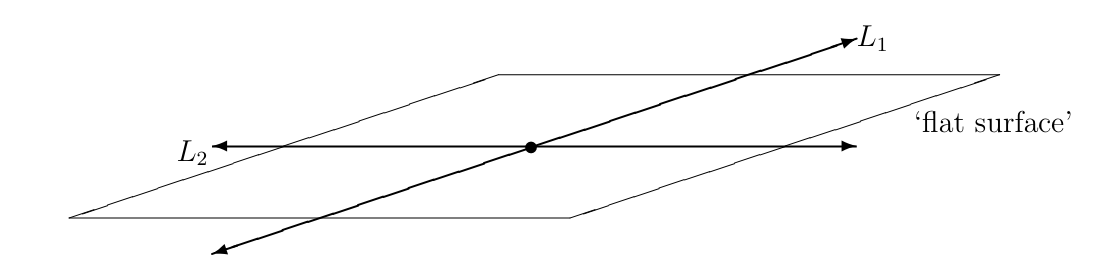
\includegraphics[width=0.7\textwidth]{figures/intersecting_lines.png}
    \caption{Two lines intersecting at a point lie on a unique plane.}
    \label{fig:intersecting-lines}
\end{figure}


  \item \textbf{Lines and Planes:} If a straight line intersects a flat surface in more than one point, then it must lie entirely within the surface. The figure below shows this situation: one line intersects the surface at a single point (and is not part of the plane), while another line intersects it in two points—indicating that it lies in the plane.
    \begin{figure}[htbp]
    \centering
    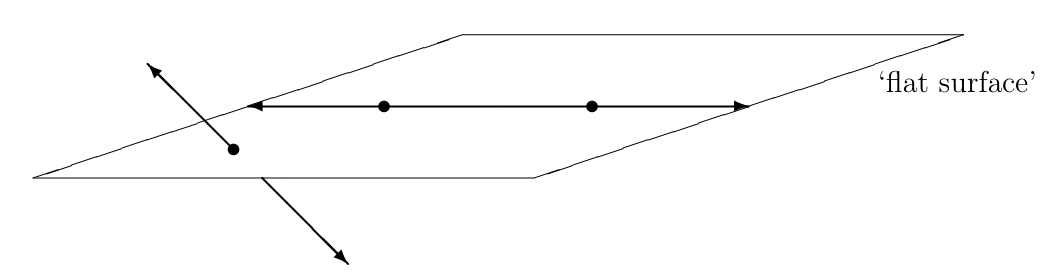
\includegraphics[width=0.7\textwidth]{figures/line_intersections_plane.png}
    \caption{A line intersecting a plane in one point vs. in two points.}
    \label{fig:line-plane-intersections}
\end{figure}

  

  \item \textbf{Three Points:} If we fix three points in space that do not all lie on the same line (i.e., they are \emph{non-collinear}), there is exactly one flat surface—one plane—that passes through all three. Imagine holding a rigid wooden board against a wall by three of its corners. The entire board is forced to lie flat against the wall; there's no room for bending. This illustrates the uniqueness of a plane determined by three non-collinear points.
        \begin{figure}[htbp]
    \centering
    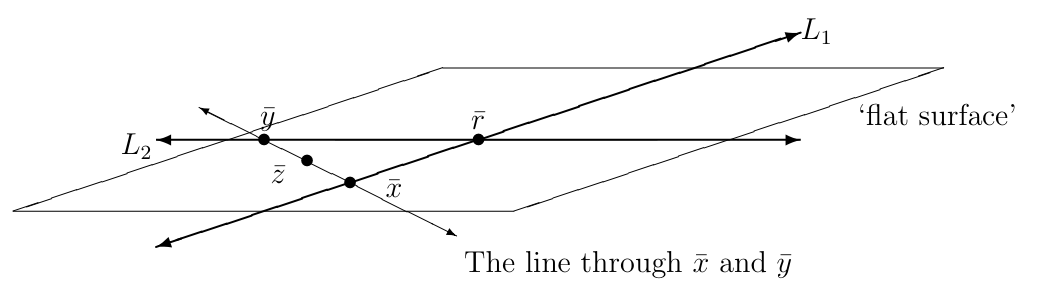
\includegraphics[width=0.6\textwidth]{figures/three_points_plane.png}
    \caption{A unique plane passes through three non-collinear points.}
    \label{fig:three-points-plane}
\end{figure}

\end{itemize}

\newpage

These intuitive ideas lead us toward a more formal definition of a plane in $\mathbb{R}^3$.

Now, suppose we are given two lines in space, $L_1$ and $L_2$, that intersect at a point $\bar{r}$. From earlier discussions (e.g., the theorem on intersecting lines), we know that these lines can be expressed parametrically as:
\[
\bar{x} = \bar{r} + t(\bar{p} - \bar{r}), \quad t \in \mathbb{R},
\]
\[
\bar{y} = \bar{r} + s(\bar{q} - \bar{r}), \quad s \in \mathbb{R},
\]
where $\bar{p} \in L_1$, $\bar{q} \in L_2$, and both pass through the common point $\bar{r}$. We now ask: what kind of surface contains \emph{every point} on both of these lines?

Take any point $\bar{x}$ on $L_1$ and any point $\bar{y}$ on $L_2$. The line connecting $\bar{x}$ and $\bar{y}$ lies in the same surface. A general point along this line can be described by:
\[
\bar{z} = \bar{x} + \alpha(\bar{y} - \bar{x}) = \bar{r} + (\alpha s)(\bar{q} - \bar{r}) + (t - \alpha t)(\bar{p} - \bar{r}), \quad \alpha \in \mathbb{R}.
\]

Thus, any such point $\bar{z}$ lies in the surface determined by $\bar{r}, \bar{p}, \bar{q}$. As we vary $s, t, \alpha \in \mathbb{R}$, we generate all points on this surface.

It appears reasonable, both geometrically and algebraically, that this set includes \emph{all} points on the plane determined by the intersecting lines $L_1$ and $L_2$.

\begin{definitionbox}

\textbf{Plane}

A \textit{plane} in \( \mathbb{R}^3 \) is a set
\[
P = \left\{ \bar{r} + s(\bar{p} - \bar{r}) + t(\bar{q} - \bar{r}) : s, t \in \mathbb{R} \right\}
\]
where \( \bar{p}, \bar{q}, \bar{r} \in \mathbb{R}^3 \) such that \( \bar{p} - \bar{r} \) and \( \bar{q} - \bar{r} \) are not scalar multiples of each other.
\end{definitionbox}

\begin{remarkbox}

Consider a set
\[
P = \left\{ \bar{r} + s(\bar{p} - \bar{r}) + t(\bar{q} - \bar{r}) : s, t \in \mathbb{R} \right\}, \quad \text{where } \bar{p}, \bar{q}, \bar{r} \in \mathbb{R}^3.
\]
\begin{enumerate}
    \item If \( \bar{p} - \bar{r} = \alpha(\bar{q} - \bar{r}) \) for some \( \alpha \in \mathbb{R} \), then
    \[
    P = \left\{ \bar{r} + s\left( \alpha(\bar{q} - \bar{r}) \right) + t(\bar{q} - \bar{r}) : s, t \in \mathbb{R} \right\}
      = \left\{ \bar{r} + (\alpha s + t)(\bar{q} - \bar{r}) : s, t \in \mathbb{R} \right\}.
    \]
    Therefore, in this case, the set \( P \) is a \textbf{line} in space.

    \item If \( \bar{p} - \bar{r} \) and \( \bar{q} - \bar{r} \) are not scalar multiples of each other, then \( P \) is a \textbf{plane} in \( \mathbb{R}^3 \). Note that:
    \[
    \bar{r} = \bar{r} + 0(\bar{p} - \bar{r}) + 0(\bar{q} - \bar{r}), \quad
    \bar{p} = \bar{r} + 1(\bar{p} - \bar{r}) + 0(\bar{q} - \bar{r}),
    \]
    \[
    \bar{q} = \bar{r} + 0(\bar{p} - \bar{r}) + 1(\bar{q} - \bar{r}).
    \]
    Thus, \( \bar{r} \in P \), \( \bar{p} \in P \), and \( \bar{q} \in P \). We therefore call \( P \) the \textbf{plane through} \( \bar{p} \), \( \bar{q} \), and \( \bar{r} \).

    \item If \( P \) is a plane, then a point \( \bar{x} \in \mathbb{R}^3 \) lies on the plane \( P \) if and only if
    \[
    \bar{x} = \bar{r} + s(\bar{p} - \bar{r}) + t(\bar{q} - \bar{r}) \quad \text{for some } s, t \in \mathbb{R}.
    \]
    We therefore speak of the plane described by the equation:
    \[
    \bar{x} = \bar{r} + s(\bar{p} - \bar{r}) + t(\bar{q} - \bar{r}).
    \]

    \item Let \( P = \left\{ \bar{r} + s(\bar{p} - \bar{r}) + t(\bar{q} - \bar{r}) : s, t \in \mathbb{R} \right\} \) be a plane through \( \bar{p}, \bar{q}, \bar{r} \), and let
    \[
    \bar{a} = \alpha(\bar{p} - \bar{r}), \quad \bar{b} = \beta(\bar{q} - \bar{r}),
    \]
    with \( \alpha, \beta \in \mathbb{R} \setminus \{0\} \). Then it follows that
    \[
    P = \left\{ \bar{r} + s\bar{a} + t\bar{b} : s, t \in \mathbb{R} \right\}.
    \]
    Conversely, if \( \bar{a}, \bar{b} \in \mathbb{R}^3 \) are nonzero vectors that are not scalar multiples of each other, then the set
    \[
    Q = \left\{ \bar{r} + s\bar{a} + t\bar{b} : s, t \in \mathbb{R} \right\}
    = \left\{ \bar{r} + s\left( (\bar{a} + \bar{r}) - \bar{r} \right) + t\left( (\bar{b} + \bar{r}) - \bar{r} \right) : s, t \in \mathbb{R} \right\}
    \]
    is a plane through the points \( \bar{r} \), \( \bar{r} + \bar{a} \), and \( \bar{r} + \bar{b} \).
\end{enumerate}
\end{remarkbox}

\begin{examplebox}
Consider the set \( P = \left\{ \langle 2, 3, -2 \rangle + s\langle 1, -4, 2 \rangle + t\langle 2, -3, 4 \rangle : s, t \in \mathbb{R} \right\} \), and
let \( \bar{r} = \langle 2, 3, -2 \rangle \), \( \bar{a} = \langle 1, -4, 2 \rangle \), and \( \bar{b} = \langle 2, -3, 4 \rangle \). Determine \( \bar{r} + \bar{a} \) and \( \bar{r} + \bar{b} \).

\vspace{0.5em}

\textbf{Solution}

\vspace{0.5em}

Since \( \bar{a} \) and \( \bar{b} \) are not scalar multiples
of each other, \( P \) is a plane through \( \bar{r} \), \( \bar{r} + \bar{a} = \langle 3, -1, 0 \rangle \), and \( \bar{r} + \bar{b} = \langle 4, 0, 2 \rangle \).
\end{examplebox}

\begin{examplebox}
Consider the set \( P = \left\{ \langle -1, 1, 6 \rangle + s\langle 2, 3, -5 \rangle + t\langle -6, -9, 15 \rangle : s, t \in \mathbb{R} \right\} \). Determine the points through which \( P \) is a line.

\vspace{0.5em}

\textbf{Solution}

\vspace{0.5em}

Since \( \langle -6, -9, 15 \rangle = -3\langle 2, 3, -5 \rangle \), we have:
\[
P = \left\{ \langle -1, 1, 6 \rangle + (s - 3t)\langle 2, 3, -5 \rangle : s, t \in \mathbb{R} \right\}
= \left\{ \langle -1, 1, 6 \rangle + \alpha\langle 2, 3, -5 \rangle : \alpha \in \mathbb{R} \right\}.
\]
Therefore, \( P \) is the line through \( \langle -1, 1, 6 \rangle \) and \( \langle 1, 4, 1 \rangle \).
\end{examplebox}

\begin{examplebox}
Consider the plane \( P = \left\{ \bar{r} + s(\bar{p} - \bar{r}) + t(\bar{q} - \bar{r}) : s, t \in \mathbb{R} \right\} \), where
\( \bar{x} = \langle 2, 0, 0 \rangle \) and \( \bar{y} = \langle 1, 2, 0 \rangle \) are given. Let \( \bar{r} = \langle 1, 1, 0 \rangle \), \( \bar{p} = \langle 0, 3, 1 \rangle \), and \( \bar{q} = \langle 1, 2, 1 \rangle \). Determine whether or not the points \( \bar{x} \) and \( \bar{y} \) lie on \( P \).

\vspace{0.5em}

\textbf{Solution}

\vspace{0.5em}

The point \( \bar{x} = \langle 2, 0, 0 \rangle \) is in \( P \) if and only if for some \( s, t \in \mathbb{R} \),
\[
\bar{x} = \bar{r} + s(\bar{p} - \bar{r}) + t(\bar{q} - \bar{r}) = \langle 1 - s, 1 + 2s + t, s + t \rangle
\]


By comparing components:
\[
\begin{aligned}
2 &= 1 - s \quad &\Rightarrow s &= -1 \\
0 &= 1 + 2s + t \quad &\Rightarrow t &= 1 \\
0 &= s + t \quad &\text{Check: } -1 + 1 = 0.
\end{aligned}
\]
So \( \bar{x} \in P \). Now check \( \bar{y} = \langle 1, 2, 0 \rangle \):
\[
\bar{y} = \bar{r} + s(\bar{p} - \bar{r}) + t(\bar{q} - \bar{r}) = \langle 1 - s, 1 + 2s + t, s + t \rangle.
\]

Compare components:
\[
\begin{aligned}
1 &= 1 - s \quad &\Rightarrow s &= 0 \\
2 &= 1 + 2s + t \quad &\Rightarrow t &= 1 \\
0 &= s + t = 0 + 1 = 1 \quad &\text{Contradiction}.
\end{aligned}
\]
Since no such \( s, t \in \mathbb{R} \) satisfy all equations, \( \bar{y} \notin P \).
\end{examplebox}

\newpage

It was mentioned at the beginning of this unit three properties that a 'flat surface' must satisfy.
We can motivate our definition of a plane in \(\mathbb{R}^3\) by showing that it satisfies the properties.

\begin{theorembox}
    \textbf{Line in a Plane}

    Let \(L\) be a line in \(\mathbb{R}^3\) and \(P\) be a plane in \(\mathbb{R}^3\) If \(L\) intersects \(P\) in more than one point,
    then \(L \subseteq P\); that is, every point on \(L\) lies on \(P\).
\end{theorembox}

\begin{proofbox}
    Let \(P = \left\{ \bar{r} + s(\bar{p} - \bar{r}) + t(\bar{q} - \bar{r}) : s, t \in \mathbb{R} \right\}\), and suppose that \(L\) intersects
    \(P\) in two points \(\bar{a} \text{ and } \bar{b}\). Then by the Theorem on Multiple Intersections of Lines,
    \[
    L = \left\{t\bar{a} + (1 - t)\bar{b} : t \in \mathbb{R}\right\}.
    \]

    Since \(\bar{a},\bar{b} \in P\), there exist distinct real numbers \(s_0,s_1,t_0,t_1\) such that
    \[
    \bar{a} = \bar{r} + s_0(\bar{p} - \bar{r}) + t_0(\bar{q} - \bar{r}) \text{ and } \bar{b} = \bar{r} + s_1(\bar{p} - \bar{r}) + t_1(\bar{q} - \bar{r}).
    \]

    Now consider a point \(\bar{x} \in L\) Then for some \(t \in \mathbb{R}\),
   \[
\begin{aligned}
\bar{x} &= t\bar{a} + (1 - t)\bar{b} \\
&= t\left[ \bar{r} + s_0(\bar{p} - \bar{r}) + t_0(\bar{q} - \bar{r}) \right] + (1 - t)\left[ \bar{r} + s_1(\bar{p} - \bar{r}) + t_1(\bar{q} - \bar{r}) \right] \\
&= [t + (1 - t)]\bar{r} + [ts_0 + (1 - t)s_1](\bar{p} - \bar{r}) + [tt_0 + (1 - t)t_1](\bar{q} - \bar{r}) \\
&= \bar{r} + [ts_0 + (1 - t)s_1](\bar{p} - \bar{r}) + [tt_0 + (1 - t)t_1](\bar{q} - \bar{r}).
\end{aligned}
\]
Hence \(\bar{x} \in P \text{ and therefore } L \subseteq P.\)
 \hfill $\qed$
\end{proofbox}
 
\begin{theorembox}

  \textbf{Unique Plane through Intersecting Lines}

  Let \(L_1\) and \(L_2\) be two lines in space that intersect at a single point. Then there is exactly one plane \(P\) that contains both lines; that is, 
  there is exactly one plane such that \(L_1 \subseteq P\) and \(L_2 \subseteq P\).

\end{theorembox}
        
\begin{proofbox}

We first show that there exists a unique plane \(P\) containing two intersecting lines \(L_1\) and \(L_2\).  

Assume \(L_1\) and \(L_2\) intersect at a point \(\bar{a}\), and let \(\bar{b} \in L_1\) and \(\bar{c} \in L_2\) be points different from \(\bar{a}\). Then, by the theorem on the intersection of lines, we hvae
\[
L_1 = \{\bar{a} + t(\bar{b}-\bar{a}) : t \in \mathbb{R}\}, \quad
L_2 = \{\bar{a} + s(\bar{c}-\bar{a}) : s \in \mathbb{R}\}.
\]

Now, consider any points \(x \in L_1\) and \(y \in L_2\). Then
\[
\bar{x} = \bar{a} + t_0(\bar{b}-\bar{a}), \quad \bar{y} = \bar{a} + s_0(\bar{c}-\bar{a})
\]
for some \(t_0, s_0 \in \mathbb{R}\). The vector connecting \(\bar{x}\) and \(\bar{y}\) is
\[
\bar{y} - \bar{x} = s_0(\bar{c}-\bar{a}) - t_0(\bar{b}-\bar{a}),
\]
which is a linear combination of \(\bar{b}-\bar{a}\) and \(\bar{c}-\bar{a}\). 

This implies that the vector connecting any point on \(L_1\) to any point on \(L_2\) lies in the span of \(\bar{b}-\bar{a}\) and \(\bar{c}-\bar{a}\). 
Consequently, if we start at \(\bar{a}\) and add all linear combinations of these two vectors, we obtain all points on \(L_1\), all points on \(L_2\), and all points “between” them. 
In other words, we obtain the entire plane containing both lines. Hence, the set
\[
P = \{\bar{a} + t(\bar{b}-\bar{a}) + s(\bar{c}-\bar{a}) : t, s \in \mathbb{R}\}
\]
contains both \(L_1\) and \(L_2\), so at least one plane containing them exists.

\vspace{1em}

Now we prove that said plane is unique.

By construction, \(\bar{b}-\bar{a}\) and \(\bar{c}-\bar{a}\) are not scalar multiples of each other, because \(L_1\) and \(L_2\) are distinct lines. 

According to the definition of a plane in \(\mathbb{R}^3\), a plane is uniquely determined by a point and two non-collinear vectors. 

Therefore, any plane containing the point \(\bar{a}\) and the vectors \(\bar{b}-\bar{a}\) and \(\bar{c}-\bar{a}\) must coincide with \(P\).  

Hence, the plane containing \(L_1\) and \(L_2\) is unique, and we have
\[
  P = \{\bar{a} + t(\bar{b}-\bar{a}) + s(\bar{c}-\bar{a}) : t, s \in \mathbb{R}\}.
\]

\hfill $\qed$

\end{proofbox}

\begin{examplebox}
  Consider the lines \(L_1\) and \(L_2\) through \(\bar{p} = \langle 1,0,1 \rangle\) and \(\bar{q} = \langle 1,2,-2 \rangle\),
  and \(\bar{u} = \langle -1,2,0 \rangle\) and \(\bar{v} = \langle -3,3,0 \rangle\).

  Show that \(L_1\) and \(L_2\) intersect, and find an equation for the plane containing both lines.

  \vspace{0.5em}

  \textbf{Solution}

  \vspace{0.5em}

  \(L_1\) and \(L_2\) intersect at \(\bar{a} = \langle x, y, z \rangle\) if and only if
  \[
    \bar{q} + t(\bar{p} - \bar{q}) = \bar{a} = \bar{u} + s(\bar{v} - \bar{u})
    \quad \text{for some } t, s \in \mathbb{R},
  \]
  \[
    \text{i.e.,}
  \]
  \[
    1 = x = 2s - 3,\quad
    2 - 2t = y = 3 - s,\quad
    2t - 1 = z = 0
    \quad \text{for some } s, t \in \mathbb{R}.
  \]
  The first equation implies \(s = 2\), and the third that \(t = \tfrac{1}{2}\).
  These values for \(s\) and \(t\) also satisfy the second equation.
  Therefore the lines \(L_1\) and \(L_2\) intersect at the point
  \[
    \bar{a} = \tfrac{1}{2} \bar{p} + \left( 1 - \tfrac{1}{2} \right) \bar{q}
    = \langle 1, 1, 0 \rangle.
  \]

  According to the Theorem on a Unique Plane through Intersecting Lines, there is exactly one plane \(P\) containing both \(L_1\) and \(L_2\).

  In order to write down an equation for this plane, we need three points on the plane that are not all on the same line.

  We have \(\bar{a} \in L_1\), \(\bar{a} \in L_2\), \(\bar{p} \in L_1\), \(\bar{u} \in L_2\).

  Since \(P\) contains \(L_1\) and \(L_2\), it follows that \(\bar{a}, \bar{p}, \bar{u} \in P\).
  
  But \(\bar{p} \notin L_2\) and \(\bar{u} \notin L_1\).
  Therefore \(\bar{a}, \bar{p}, \bar{u}\) are not all on the same line.

  Hence an equation for \(P\) is
  \[
    \bar{x} = \bar{a} + s(\bar{p} - \bar{a}) + t(\bar{u} - \bar{a})
    = \langle 1, 1, 0 \rangle + s\langle 0, -1, 1 \rangle + t\langle -2, 1, 0 \rangle.
  \]
\end{examplebox}


\begin{theorembox}

  \textbf{Three-Point Plane Theorem}

  Let \(\bar{p}, \bar{q}\) and \(\bar{r}\) be three points in \(\mathbb{R}^3\), not all on the same line. 
  Then there exists a unique plane \(P \in \mathbb{R}^3\) such that \(\bar{p}, \bar{q}, \bar{r} \in P\).
\end{theorembox}

\begin{proofbox}
  Let \(L_1\) be the line through \(\bar{p}\) and \(\bar{r}\), and \(L_2\) be the line through \(\bar{q}\) and \(\bar{r}\).

  \vspace{0.5em}

  Since \(\bar{p}, \bar{q}\) and \(\bar{r}\) are not all on the same line, it follows that \(L_1\) and \(L_2\) intersect at a single point, namely, at \(\bar{r}\).
  It follows from the Theorem on a Unique Plane through Intersecting Lines that there exists a unique plane \(P\) containing both \(L_1\) and \(L_2\).

  \vspace{0.5em}

  Since \(\bar{p},\bar{r} \in L_1\) and \(\bar{q},\bar{r} \in L_2\), it follows that \(\bar{p},\bar{q},\bar{r} \in P\).

  \vspace{0.5em}

  If some plane \(Q\) is a plane containing \(\bar{p},\bar{q},\) and \(\bar{r}\), then \(L_1,L_2 \subseteq Q\) by the Theorem on a Line in a Plane
  Since \(P\) is the unique plane containing both \(L_1\) and \(L_2\), it follows that \(P = Q\). 

  \hfill \(\qed\)

\end{proofbox}

\newpage

Recall that we call two lines \(L_1 = \{\bar{q} + t(\bar{p} - \bar{q}) : t \in \mathbb{R}\}\) and \(L_2 = \{\bar{r} + s(\bar{q} - \bar{r}) : s \in \mathbb{R}\}\)
\textit{parallel} if \(\bar{p} -\bar{q}\) and \(\bar{a}-\bar{b}\) are scalar multiples of each other. We showed in the Theorem on the Non-Intersection of Parallel Lines that
if \(L_1\) and \(L_2\) are parallel, and \(L_1 \neq L_2\), then \(L_1\) and \(L_2\) do not intersect. The converse of this statement is false-in the example that followed, we showed an instance
of two lines that are not parallel, and do not intersect. 

The following result further clarifies this issue.

\begin{theorembox}

  \textbf{Parallel Lines in a Plane}

Let \(L_1\) and \(L_2\) be two lines in \(\mathbb{R}^3\) such that \(L_1 \neq L_2\) defined as

\[
  L_1 = \{\bar{q} + t(\bar{p} - \bar{q}) : t \in \mathbb{R}\}, \quad
  L_2 = \{\bar{r} + s(\bar{q} - \bar{r}) : s \in \mathbb{R}\}.
\]

Then the following statements are true:
\begin{enumerate}[label=(\arabic*)]
  \item If \(L_1\) and \(L_2\) are parallel, then there exists exactly one plane \(P\) that contains both lines.
  \item If \(L_1\) and \(L_2\) do not intersect, and there is a plane \(P\) such that \(L_1,L_2 \subseteq P\), then \(L_1\) and \(L_2\) are parallel.
\end{enumerate}
\end{theorembox}

\begin{proofbox}

  \begin{enumerate}[label=(\arabic*), series = ParLinProof]
    \item Assume that \(L_1\) and \(L_2\) are parallel. Then by the definition of parallel lines, there exists a non-zero \(\alpha \in \mathbb{R}\) such that

    \[
      \bar{a} - \bar{b} = \alpha(\bar{p} - \bar{q}).
    \]

    Since \(L_1\) and \(L_2\) are parallel, it follows by the Theorem on Non-Intersection of Parallel Lines, that \(L_1\) and \(L_2\) do not intersect.

    Therefore \(\bar{p},\bar{q}, \bar{b}\) are not all on the same line. By the Three-Point Plane Theorem, we find that

    \[
      P = \{\bar{q} + s(\bar{p} - \bar{q}) + t(\bar{b} - \bar{q}) : s, t \in \mathbb{R}\}.
    \]
    is a plane in \(\mathbb{R}^3\) such that \(\bar{p}, \bar{q}, \bar{b} \in P\).

    Now consider points \(\bar{x}\) and \(\bar{y}\) on \(L_1\) and \(L_2\), respectively.

    Then
    \[
      \bar{x} = \bar{q} + t(\bar{p} - \bar{q}), \quad
      \bar{y} = \bar{r} + s(\bar{q} - \bar{r}) \text{ for some s,t } \in \mathbb{R}.
    \]


  \end{enumerate}
\end{proofbox}